\begin{frame}
\frametitle{About This Work...}

\emph{Cleaning Trajectory Data of RFID-monitored Objects through Conditioning under Integrity}~\cite{DBLP:conf/edbt/FazzingaFFP14}\\
B.~Fazzinga, S.~Flesca, F.~Furfaro, F.~Parisi.\\~\\

% \emph{Handling False Negatives in Indoor RFID Data}.~\cite{baba2014handling} \\
% A.I.~Baba, H.~Lu, T.B.~Pedersen, X.~Xie\\~\\

\begin{itemize}
  \item Published at \emph{EDBT' 2014}. %, \emph{MDM' 2014}.
  \item A probabilistic framework is introduced for reducing the inherent uncertainty of trajectory data collected for RFID-monitored objects.
  \item The framework cleans trajectories by conditioning them to the event that integrity constraints encoding some knowledge about the map and the motility characteristics of the monitored objects hold.
\end{itemize}

\end{frame}

%------------------------------------------------

\begin{frame}
\frametitle{Motivation}

\begin{itemize}
  \item Pervasive use of RFID devices as a support for object tracking
  \begin{fitemize}
    \item monitoring of people, animals and objects inside museums, shools, hospital etc.
    \item context-aware information.
  \end{fitemize}
  \item There exists ambiguity in the raw RFID data.
  \begin{fitemize}
    \item no one-to-one correspondence between locations and readers, no way to deterministically decide the location given that a set of readers detected an object.
    \item the same location may constain different reader's detection zones, the same reader may detect different objects at different locations, also false negatives.
  \end{fitemize}
\end{itemize}

\end{frame}

%------------------------------------------------

\begin{frame}
\frametitle{Ambiguity of RFID Data}

\begin{columns}

  \column{0.4\textwidth}
  \begin{figure}[tb]
    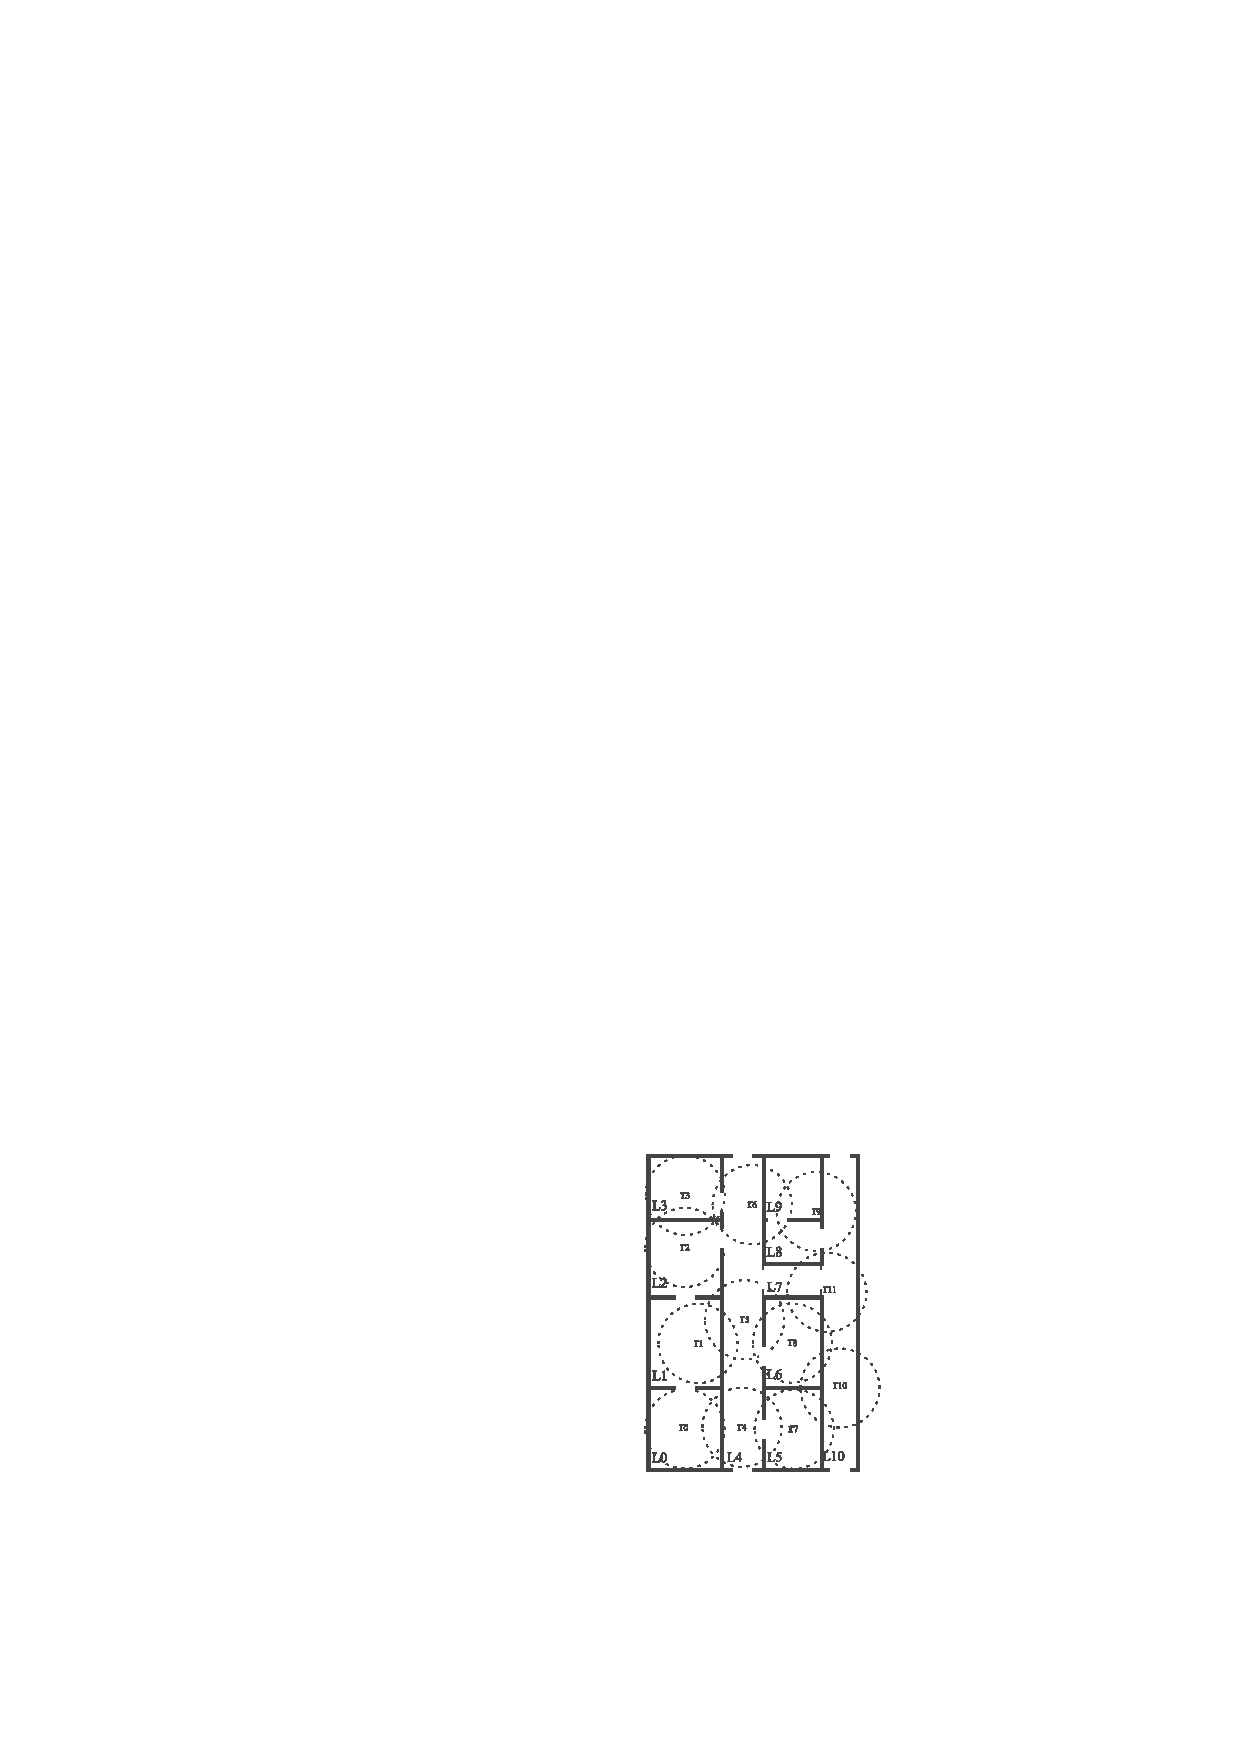
\includegraphics[width=\columnwidth]{figures/3-4/3-4-1.pdf}
  \end{figure}

  \column{0.6\textwidth}
  \begin{example}
    \fsize{
    an object $o$ was detected at some instant by both reader $r_1$ and $r_5$, two locations are possible, $L_1$ and $L_4$. Analogously, if $o$ was detected by $r_3$ only, we cannot conclude that it was surely in $L_3$, as it could be the case that $r_2$ failed to detect it despite it was close enough to its antenna.
    }
  \end{example}

  \ssize{\textrm{\\this suggests that the association readers/locations can be naturally modeled in probabilistic terms. For instance by a probability distribution $p^a(l|R)$ defined for each location $l$ and set $R$ of readers.}}
  $p^a(L_1|\{r_1, r_5\}) = p^a(L_4|\{r_1, r_5\}) = 0.5$
  $p^a(L_0|\{r_0\}) = 1$

\end{columns}

\end{frame}

%------------------------------------------------

\begin{frame}
\frametitle{Ambiguity of RFID Data}

\begin{columns}

  \column{0.4\textwidth}
  \begin{figure}[tb]
    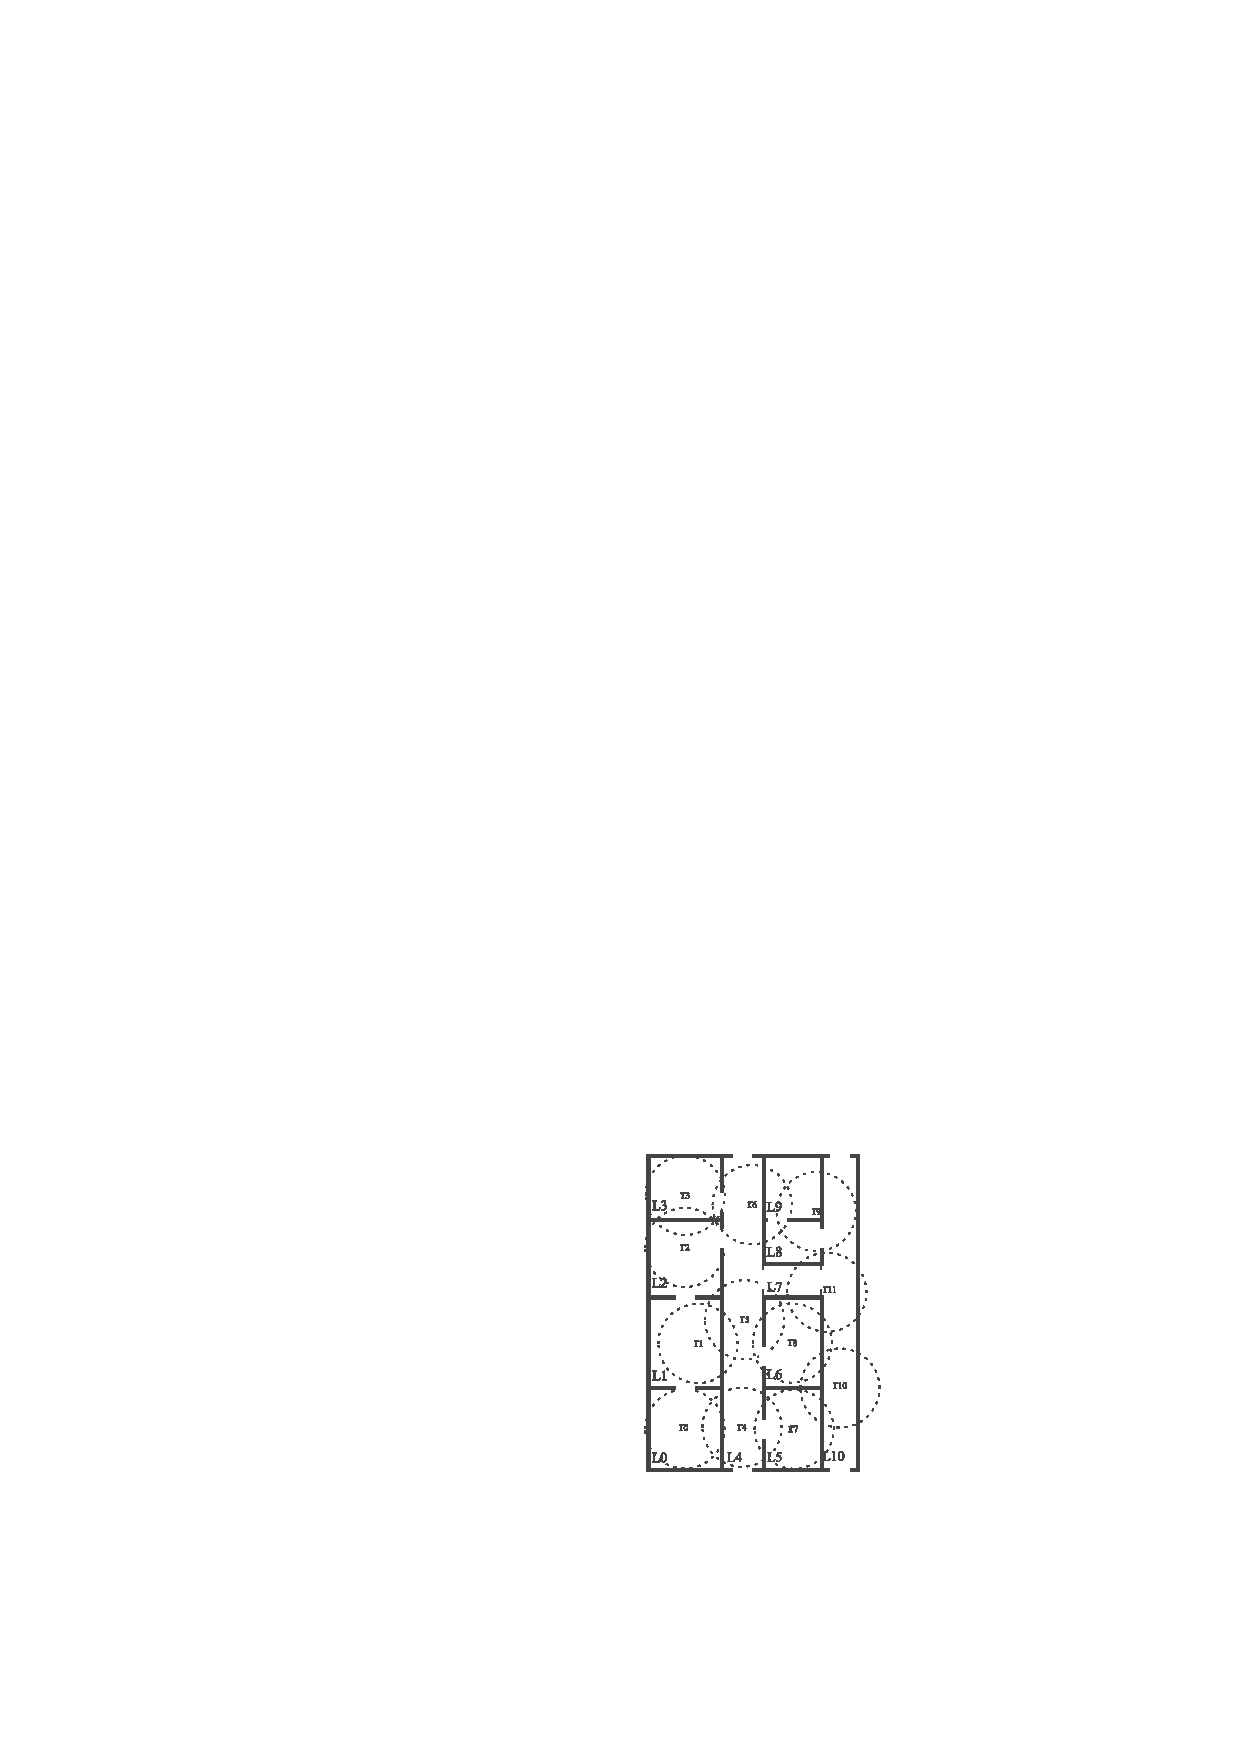
\includegraphics[width=\columnwidth]{figures/3-4/3-4-1.pdf}
  \end{figure}

  \column{0.6\textwidth}
  \ssize{\textrm{things become more complex when trying to translate a sequence of readings into possible trajectories, a naive way is to consider the steps of the trajectory independent from each other.}}

  \begin{example}
    \ssize{
    assume that at instants(timestamps) 0 and 1, $o$ is detected by both $r_1$ and $r_5$, while at instant 2 it's detected by $r_0$. Assume that $p^a(l|R)$ is used, i.e., objects detected by $r_1$ and $r_5$ are at location $L_1$ with probability 0.5 and at $L_4$ with probability 0.5, detected by $r_0$ are at $L_0$ with probability 1. Reasoning only on the basis of these probabilities and exploiting no further knowledge, the trajectories followed by $o$ can be: $t_1: L_1L_1L_0$, $t_2: L_1L_4L_0$, $t_3: L_4L_1L_0$, $t_4: L_4L_4L_0$, each with pribability 0.25.
    }
  \end{example}

\end{columns}

\end{frame}

%------------------------------------------------

\begin{frame}
\frametitle{Ambiguity of RFID Data}

The independence assumption allows for reasoning about tracjectory probabilities as follows.\\~\\
\pause

Consider an object $o$ moving over time interval $\mathcal{T} = [\tau_1,...,\tau_n]$, and the sequence of readings $\Theta = \langle \tau_1, R_1 \rangle, ..., \langle \tau_n, R_n \rangle$, meaning that at each $\tau_i \in \mathcal{T}$, $o$ was detected by the set $R_i$ of readers.\\~\\
\pause

The probability that $o$ followed the trajectory $t = l_1, ..., l_n$ can be expressed (under the independence assumption) as $p^a(t|\Theta) = \prod_{i=1}^n p^a(l_i|R_i)$.\\~\\
\pause

Unfortunately, the probabilities returned by $p^a(t|\Theta)$ can be very different from those returned by the ``actual'' probability distribution $Pr(t|\Theta)$ as the following example.

\end{frame}

%------------------------------------------------

\begin{frame}
\frametitle{Ambiguity of RFID Data}

\begin{columns}

  \column{0.4\textwidth}
  \begin{figure}[tb]
    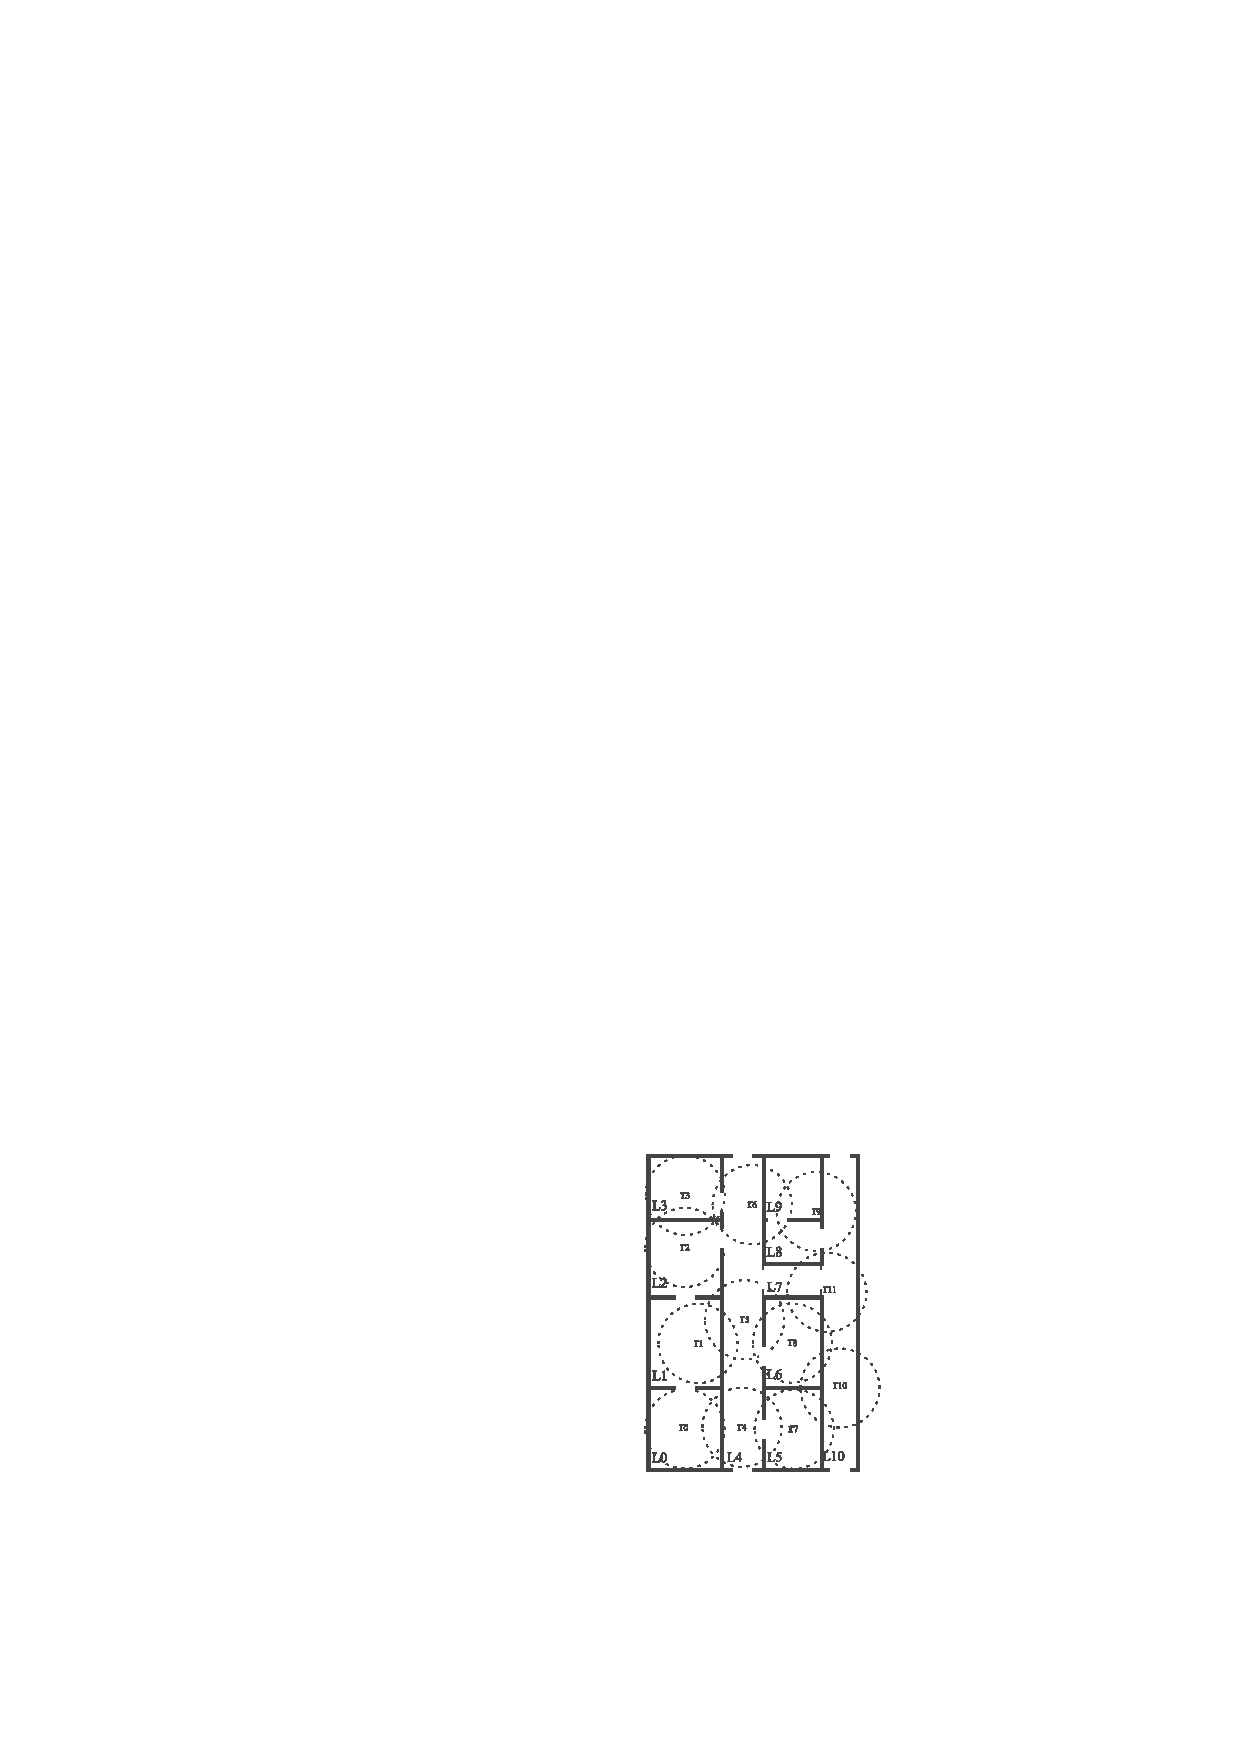
\includegraphics[width=\columnwidth]{figures/3-4/3-4-1.pdf}
  \end{figure}

  \column{0.6\textwidth}

  \begin{example}
    \ssize{
    For the four possible trajectories $t_1: L_1L_1L_0$, $t_2: L_1L_4L_0$, $t_3: L_4L_1L_0$, $t_4: L_4L_4L_0$, we can infer only $t_1$ is the only correct interpretation of the data according to the map. Since $L_0$ and $L_4$ have no direct connection, and $L_1$ is directly connected to $L_0$ by not to $L_4$. Thus a correct probability distribution over the possible trajectories is at follows: $Pr(t_1|\Theta) = 1$, $Pr(t_2|\Theta) = Pr(t_3|\Theta) = Pr(t_4|\Theta) = 0$, where $\Theta = \theta_1, \theta_2$, and $\theta_1 = \langle \tau_1, \{ r_1, r_5 \} \rangle $, $\theta_2 = \langle \tau_2, \{ r_0 \} \rangle $.
    }
  \end{example}

  \ssize{\textrm{the point is that even $p^a(l|R)$(also $p^a(t|\Theta)$) is easy to obtain, finding a formulation for $Pr(t|\Theta)$ is very hard, as it requires analyzing and encoding the correlations among possible positions over time.}}

\end{columns}

\end{frame}

%------------------------------------------------

\begin{frame}
\frametitle{Target of This Work}

\begin{problem}
  given a sequence of readings $\Theta$ and exploiting the knowledge of $p^a(l|R)$ (and thus $p^a(t|\Theta)$), how can we effectively and efficiently revise $p^a(t|\Theta)$ so that it takes into account possible correlations inside the data, thus obtaining a better estimate of $Pr(t|\Theta)$.
\end{problem}

Intuitively enough, revising $p^a(t|\Theta)$ according to the known correlations can be viewed as a cleansing problem: the data to be cleaned are the (probabilistic) trajectories resulting from using $p^a(t|\Theta)$ to interpret the sequence of readings, and the cleansing task consists in revising the probablitisties assigned to these trajectories.

\end{frame}

%------------------------------------------------

\begin{frame}
\frametitle{Cleansing RFID Data}

Exploiting the knowledge on the map and on the motility characteristics:\\~\\

\conceptbf{Direct-unreachability Constraint} can be naturally derived on the connectivity between pairs of locations.\\~\\

\conceptbf{Traveling-time Constraint} can be derived on the time needed for reaching a location starting from another one.

\end{frame}

%------------------------------------------------

\begin{frame}
\frametitle{Cleansing RFID Data}

\begin{columns}

  \column{0.4\textwidth}
  \begin{figure}[tb]
    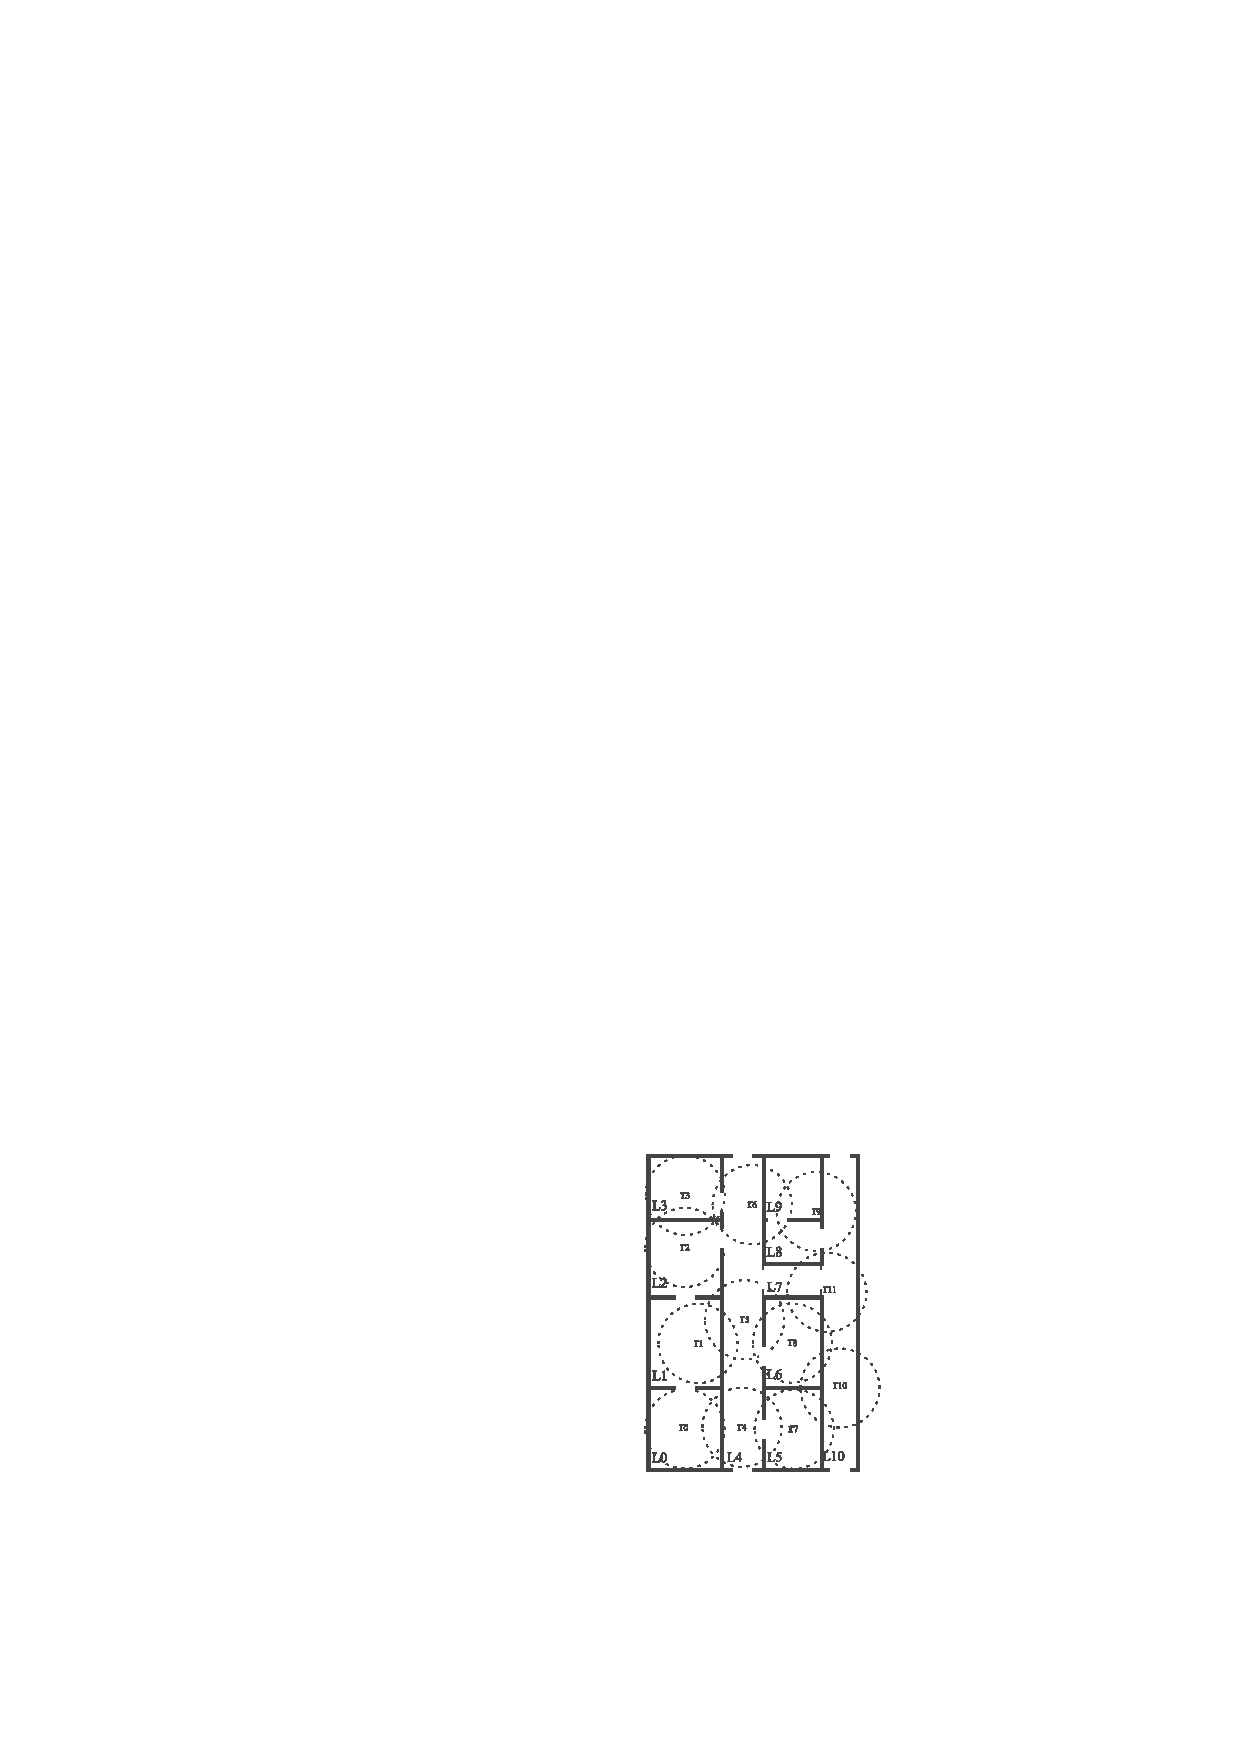
\includegraphics[width=\columnwidth]{figures/3-4/3-4-1.pdf}
  \end{figure}

  \column{0.6\textwidth}

  \begin{example}
    \ssize{
      the map easily implies a set of direct-unreachability constraints, one for each pair of rooms which are not directly connected through a door, such as $L_0,L_4$ and $L_1,L_4$.\\
      The map implies further constraints, other than direct unreachability. E.g., it says that $L_0$ and $L_5$, althrough close to one another, are connected only by a pretty long path. Reasonably, it can be imposed that $15 sec$ are required to go through this path. (called ``traveling-time constraint'').
    }
  \end{example}
  \ssize{\textrm{the above example explains how considering integrity constraints can reduce uncertainty, as it allows trajectories to be removed from the valid interpretations of data.}}

\end{columns}

\end{frame}

%------------------------------------------------

\begin{frame}
\frametitle{Cleansing RFID Data}

\fsize{

\conceptbf{The target of this work} becomes how to reasonably combine the integrity constraints with the \emph{a-priori} probabilistic model encoded by $p^a(l|R)$, in order to devise a mechanism for revising the a-priori probabilities of the remaing valid trajectories and making them sum up to 1.\\~\\

A rigorous approach~\cite{koch2008conditioning,flesca2014consistency} is to perform \conceptbf{conditioning}: starting from the a-priori probabilities(without constraints), the probabilities of the trajectories are re-evaluated as conditioned to the event that the constraints are satisfied.\\~\\

That is, given a set $\mathcal{IC}$ constraints, probabilities of the form $p^a(t|\Theta)$ are revised into $p^a(t|\Theta \wedge \mathcal{IC})$. This way, the probability of invalid trajectories becomes 0, while that of each valid trajectory becomes the ratio of its a-priori probability to the overall a-priori probability of the valid trajectories.

}

\end{frame}

%------------------------------------------------

\begin{frame}
\frametitle{Preliminaries}

\ssize{
\begin{table}
    \begin{center}
    \begin{tabular}{|c|c|}
    \hline
        \textbf{Notation} &   \textbf{Meaning}                    \\
    \hline
        $o$      &   a single object equipped with RFID tag        \\
    \hline
        $\mathcal{R} = \{ r_1, ..., r_k \}$      &   a set of RFID readers     \\
    \hline
        $\mathcal{L} = \{ l_1, ..., l_n \}$      &  the set of locations       \\
    \hline
        $\mathcal{T} = [0..\tau_f]$      &  the time interval over monitoring       \\
    \hline
        $\theta = \langle \tau, R \rangle$      &  a reading of $o$ \\
    \hline
        $\Theta$        &   a set of readings, a \emph{reading sequence} (r-sequence) \\
    \hline
        $p^a(l|R)$        &   the \emph{a-priori} probability  \\
    \hline
        $X_{\theta}$        &   the discrete random variable \\
    \hline
        $f(X_{\theta} = l) = p^a(l|\theta[readers])$        &   probability density funtion for the random variable \\
    \hline
    \end{tabular}
    \end{center}
\end{table}
}

\end{frame}

%------------------------------------------------

\begin{frame}
\frametitle{Preliminaries}

\begin{definition}[probabilistic location sequence (l-sequence)]
  given $p^a(l|R)$ and an r-sequence $\Theta$, we define the \emph{probabilistic location sequence} corresponding to $\Theta$ (according to $p^a(l|R)$) as the set $\Gamma = \{ X_{\theta} | \theta \in \Theta \}$.
\end{definition}

\fsize{
The l-sequence $\Gamma$ corresponding to the r-sequence $\Theta$ for $o$ over $\mathcal{T}$ will be denoted as a pair $\Gamma = \langle \Lambda,p \rangle$.
\begin{itemize}
  \item $\Lambda$ is a set of pairs of the form $\Lambda = \langle \tau, l \rangle$, with $\tau \in \mathcal{T}$ and $l \in \mathcal{L}$, containing at least one pair $\langle \tau, l \rangle$ for each $\tau \in \mathcal{T}$.
  \item $p$ assigns to each pair $\langle \tau, l \rangle \in \Lambda$ the value $f(X_{\theta} = l)$, where $\theta$ is the reading at time $\tau$, i.e., $p$ assigns to $\langle \tau, l \rangle$ the probability that the object was at location $l$ at time $\tau$, as implied by the PDF of the random variable.
\end{itemize}
}

\end{frame}

%------------------------------------------------

\begin{frame}
\frametitle{Preliminaries}

\begin{columns}

  \column{0.4\textwidth}
  \begin{figure}[tb]
    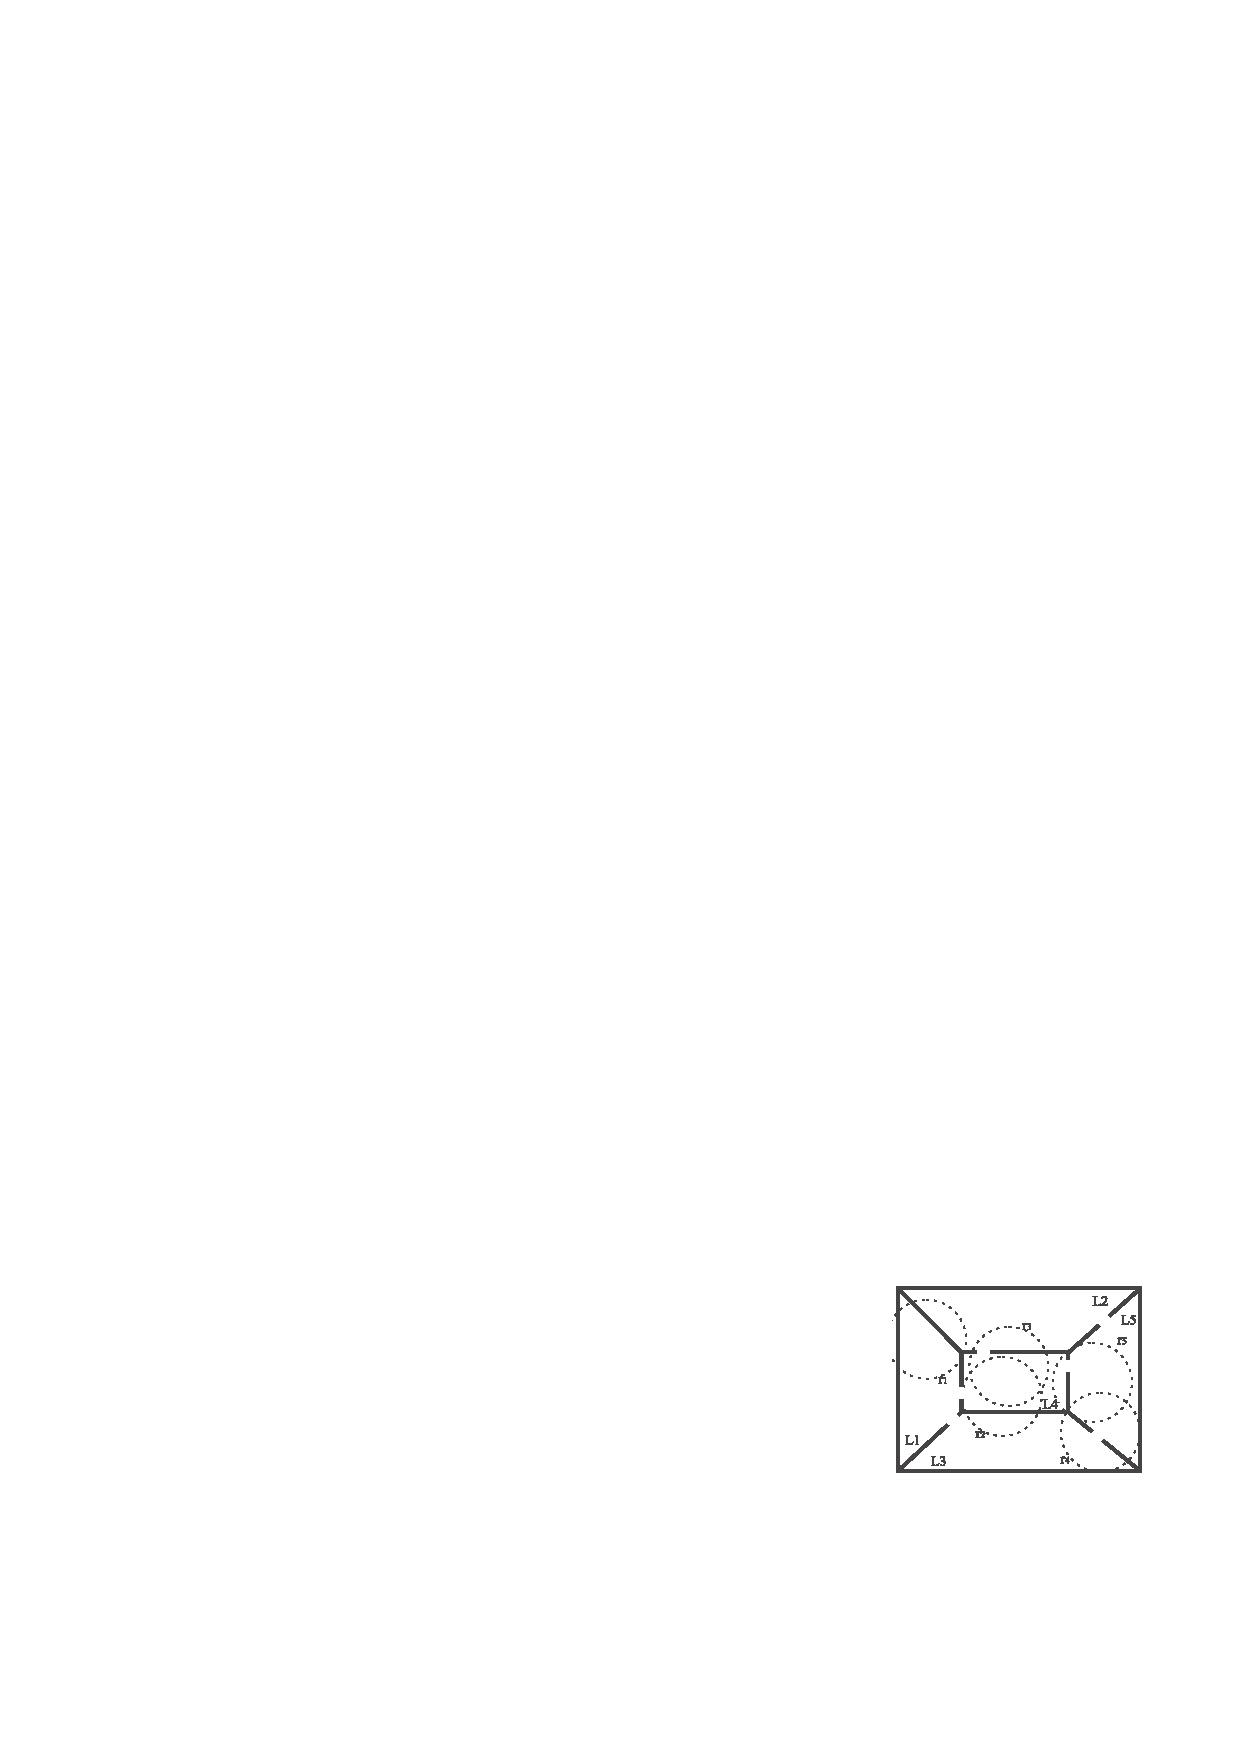
\includegraphics[width=\columnwidth]{figures/3-4/3-4-2.pdf}
  \end{figure}

  \column{0.6\textwidth}

  \begin{example}
    \ssize{
      consider the r-sequence $\Theta = \{ \langle 0, \{ r_1 \} \rangle, \langle 1, \{ r_2 \} \rangle, \langle 2, \{ r_4 \} \rangle \}$ and $p^a(l|R)$ s.t. $p^a(L_1|\{r_1\}) = \frac{6}{10}$, $p^a(L_2|\{r_1\}) = \frac{4}{10}$, $p^a(L_3|\{r_2\}) = \frac{1}{3}$, $p^a(L_4|\{r_2\}) = \frac{2}{3}$, $p^a(L_3|\{r_4\}) = \frac{2}{3}$, $p^a(L_5|\{r_4\}) = \frac{1}{3}$. The corresponding l-sequence $ \Gamma = \langle \Lambda, p \rangle $ is s.t. $ \Lambda = \{ \lambda_1 = \langle 0, L_1 \rangle, \lambda_2 = \langle 0, L_2 \rangle, \lambda_3 = \langle 1, L_3 \rangle, \lambda_4 = \langle 1, L_4 \rangle, \lambda_5 = \langle 2, L_3 \rangle, \lambda_6 = \langle 2, L_5 \rangle \} $, and $p(\lambda_1) = \frac{6}{10}$, $p(\lambda_2) = \frac{4}{10}$, $p(\lambda_3) = \frac{1}{3}$, $p(\lambda_4) = \frac{2}{3}$, $p(\lambda_5) = \frac{2}{3}$, $p(\lambda_6) = \frac{1}{3}$.
    }
  \end{example}

\end{columns}

\end{frame}

%------------------------------------------------

\begin{frame}
\frametitle{Preliminaries}

given a pair $\lambda = \langle \tau, l \rangle \in \Lambda$, denote the first and the second component of $\lambda$ with $\lambda[time]$ and $\lambda[loc]$ respectively.

\begin{definition}[Trajectory]
  Let $\Theta$ be an r-sequence over $\mathcal{T}$ and $\Gamma = \langle \Lambda,p \rangle$ be the l-sequence corresponding to $\Theta$. A trajectory over $\Gamma$ is a set $t \subseteq \Lambda$ of pairs such that, for each $\tau \in \mathcal{T}$, there is a unique pair $\lambda \in t$ such that $\lambda[time] = \tau$. The (a-priori) probablitity of $t$ is $p^a(t|\Theta) = \prod_{\lambda \in t}p(\lambda)$. For simplicity, we write $p^a(t|\Theta)$ as $p^a(t)$.
\end{definition}

The set of the trajectories over an l-sequence $\Gamma$ is denoted as $T(\Gamma)$. Given a trajectory $t$, the pair $\lambda \in t$ such that $\lambda[time] = \tau$ is said to be the $\tau$-th \emph{step} of $t$.

\end{frame}

%------------------------------------------------

\begin{frame}
\frametitle{Preliminaries}

\begin{columns}

  \column{0.4\textwidth}
  \begin{figure}[tb]
    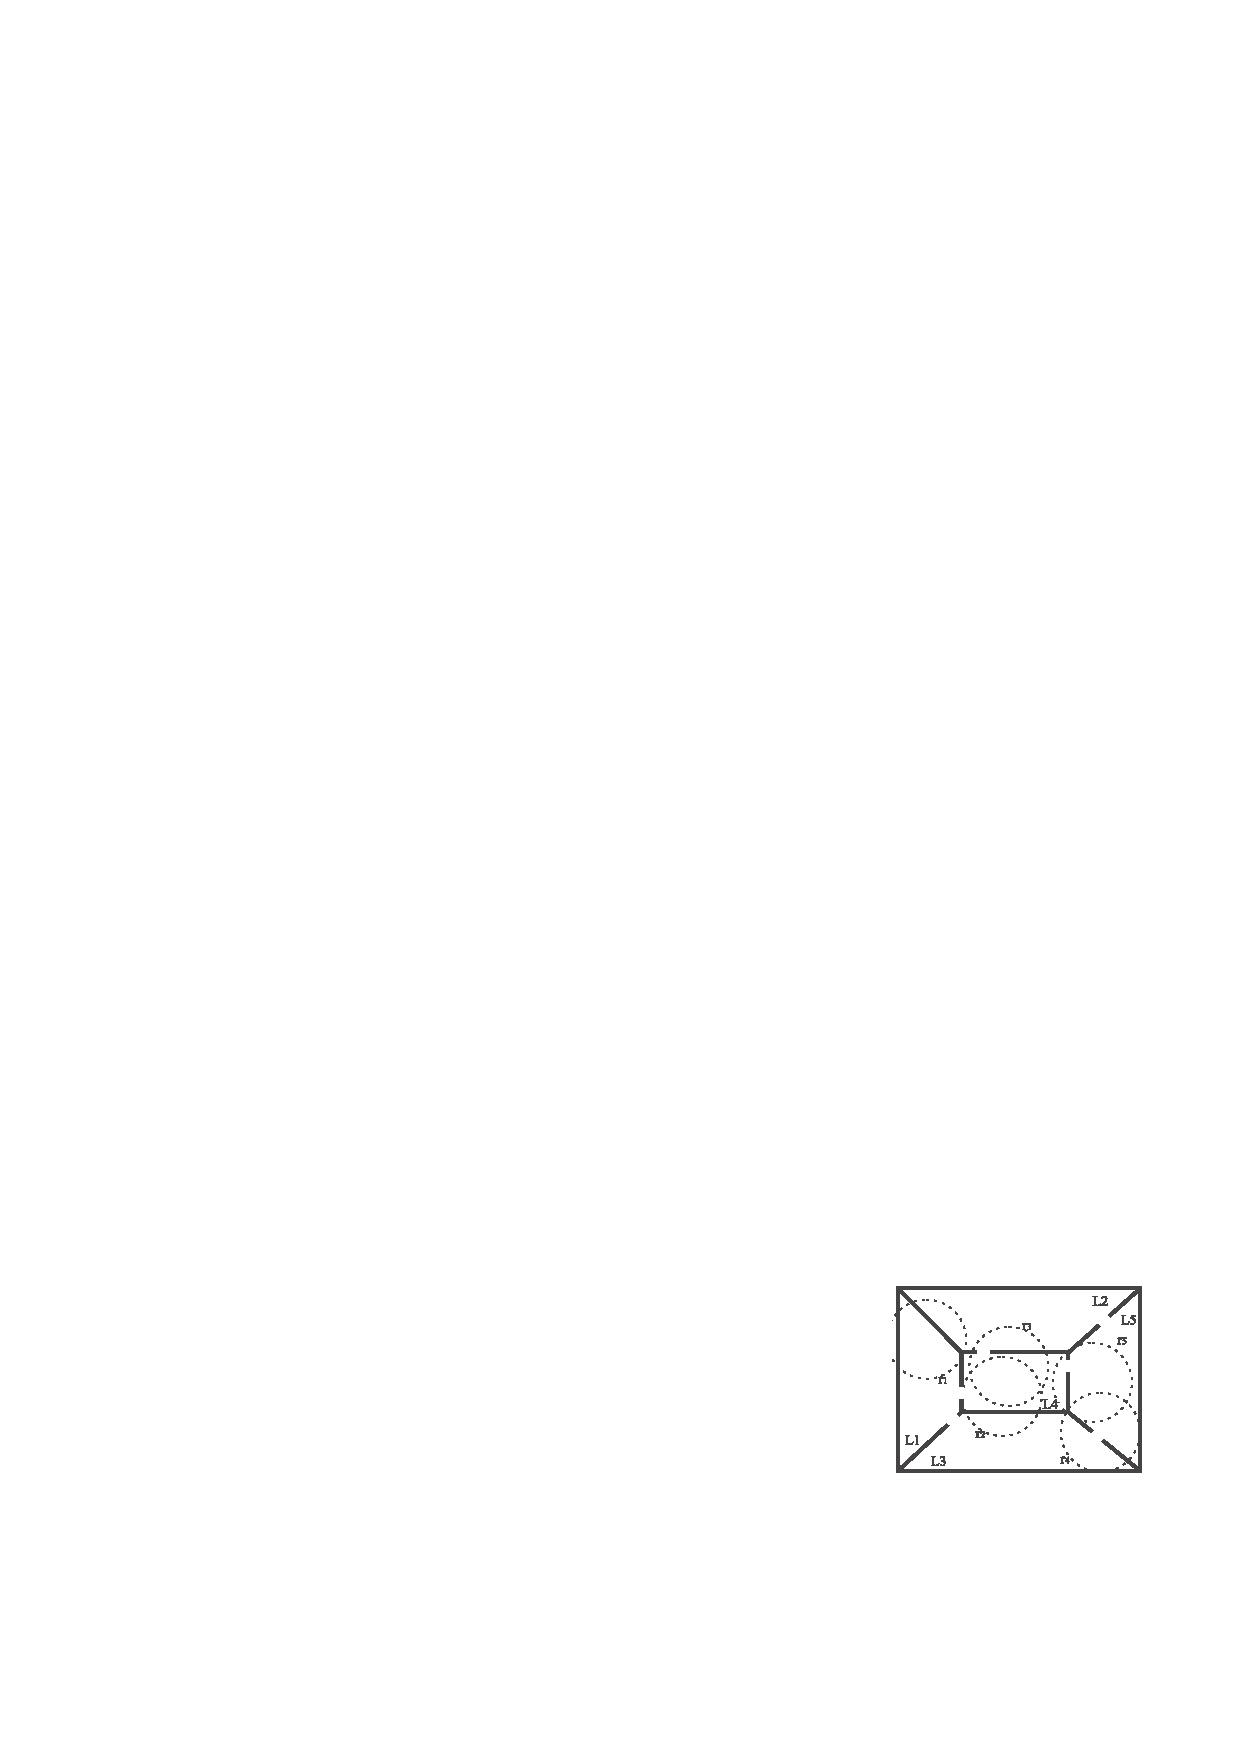
\includegraphics[width=\columnwidth]{figures/3-4/3-4-2.pdf}
  \end{figure}

  \column{0.6\textwidth}

  \begin{example}
    \ssize{
      2 out of the 8 trajectories over the l-sequence $\mathcal{T} = \langle \Lambda,p \rangle$ are $t_1 = \{\lambda_1, \lambda_3, \lambda_5\}$, which means that object $o$ went from $L_1$ to $L_3$ and stayed in $L_3$ for two consecutive timestamps, and $t_2 = \{\lambda_1, \lambda_3, \lambda_6\}$, which describes the case that object $o$ went from $L_1$ to $L_5$ through $L_3$. Their a-priori probabilities are $p^a(t_1) = p(\lambda_1) \cdot p(\lambda_3) \cdot p(\lambda_5) = \frac{12}{90}$, and $p^a(t_2) = p(\lambda_1) \cdot p(\lambda_3) \cdot p(\lambda_6) = \frac{6}{90}$.

    }
  \end{example}

\end{columns}

\end{frame}
